
\begin{center}
\Huge
	Trigonometriske funktioner
\end{center}
\section*{Radianer}
\stepcounter{section}

I trigonometriforløbet har vi arbejdet med de trigonometriske funktioner cosinus, sinus og tangens den kontekst, at de skal hjælpe os med at bestemme vinkler og sider i trekanter. Vi vil i dette forløb betragte dem mere som funktioner, der i sig selv har interesse. 

Når vi taler om trigonometriske funktion som funktioner, så vil vi i stedet for grader typisk anvende det, vi kalder \textit{radianer}. Enhedscirklen har som bekendt en omkreds på $2\pi$ og radianer tilsvarer den andel af cirkelbuen, en vinkel dækker over i enhedscirklen. Vi kan se det visualiseret på Figur \ref{fig:radian}.
\begin{figure}[H]
	\centering
	\begin{tikzpicture}
	\begin{axis}
		[
		axis lines = center, 
		xmin = -1.3, xmax = 1.4,
		ymin = -1.3, ymax = 1.4,
		x = 4cm, y = 4cm,
		ticks = none
		]
		\draw[thick, color = teal] (axis cs: 0,0) circle (4cm);
		\draw[color = teal, thick] (axis cs: 0,0) -- (axis cs: {cos(50},{sin(50)});
		\draw[color = purple, thick] (axis cs: 0.15,0) arc[start angle = 0, end angle = 50, radius = 0.15*4cm];
		\node[color = purple, anchor = west] at (axis cs: 0.2,0.1) {$v$ i grader};
		\draw[color = purple, thick] (axis cs: 1.05,0) arc[start angle = 0, end angle = 50, radius = 1.05*4cm]
		node[midway, anchor = south, rotate = -65] {$v$ i radianer};
		\draw[color = purple, thick] (axis cs: {1.03*cos(0)}, {1.03*sin(0)} )
		 -- (axis cs: {1.07*cos(0)}, {1.07*sin(0)} );
		 \draw[color = purple, thick] (axis cs: {1.03*cos(50)}, {1.03*sin(50)} )
		 -- (axis cs: {1.07*cos(50)}, {1.07*sin(50)} );
		\node[anchor = north west] at (axis cs: 1,0) {$1$};
		\node[anchor = south west] at (axis cs: 0,1) {$1$};
	\end{axis}
	\end{tikzpicture}
	\caption{Radianer og vinklers sammenhæng}
	\label{fig:radian}
\end{figure}
\newpage
\begin{exa}
	Vi betragter vinklen $60^\circ$ på Figur \ref{fig:exa1}.
	\begin{figure}[H]
	\centering
	\begin{tikzpicture}
	\begin{axis}
		[
		axis lines = center, 
		xmin = -1.3, xmax = 1.4,
		ymin = -1.3, ymax = 1.4,
		x = 4cm, y = 4cm,
		ticks = none
		]
		\draw[thick, color = teal] (axis cs: 0,0) circle (4cm);
		\draw[color = teal, thick] (axis cs: 0,0) -- (axis cs: {cos(15},{sin(15)});
		\draw[color = teal, thick] (axis cs: 0,0) -- (axis cs: {cos(75},{sin(75)});
		\draw[color = purple, thick] (axis cs: {0.15*cos(15)},{0.15*sin(15)})
		 arc[start angle = 15, end angle = 75, radius = 0.15*4cm];
		\node[color = purple, anchor = south west, rotate = 0] at (axis cs: 0.1,0.1) {$60^\circ$};
		\draw[color = purple, thick] (axis cs: {1.05*cos(15)}, {1.05*sin(15)})
		 arc[start angle = 15, end angle = 75, radius = 1.05*4cm]
		 node[midway, rotate = 0, anchor = south west] {$\frac{\pi}{3}$};
		\draw[color = purple, thick] (axis cs: {1.03*cos(15)}, {1.03*sin(15)} )
		 -- (axis cs: {1.07*cos(15)}, {1.07*sin(15)} );
		 \draw[color = purple, thick] (axis cs: {1.03*cos(75)}, {1.03*sin(75)} )
		 -- (axis cs: {1.07*cos(75)}, {1.07*sin(75)} );
		\node[anchor = north west] at (axis cs: 1,0) {$1$};
		\node[anchor = south west] at (axis cs: 0,1) {$1$};
	\end{axis}
	\end{tikzpicture}
	\caption{$60^\circ$ som radianer.}
	\label{fig:exa1}
\end{figure}
	Vi skal omregne $60^\circ$ til radianer. Vi begynder med at dele med $360$ for at finde ud af, hvor stor en andel af 
	cirklen, $60^\circ$ tilsvarer. Vi får da 
	\begin{align*}
		\frac{60}{360} = \frac{1}{6}.
	\end{align*}
	Da der i enhedscirklen er $2\pi$ radianer hele vejen rundt, ganger vi derfor med $2\pi$. 
	\begin{align*}
		\frac{1}{6}\cdot 2\pi = \frac{\pi}{3}.
	\end{align*}
	$60^\circ$ tilsvarer altså $\frac{\pi}{3}$ radianer. 
\end{exa}
\begin{exa}
	Vi kan selvfølgelig også regne den anden vej. Lad os sige, at vi har en vinkel på $\frac{11\pi}{12}$ i radianer. Vi 
	deler tilsvarende med $2\pi$ først.
	\begin{align*}
		\frac{11\pi}{12\cdot 2\pi} = \frac{11}{24}.
	\end{align*}
	Vi ganger så med $360$ for at få resultatet i grader.
	\begin{align*}
		\frac{11\cdot 360}{24} = 11\cdot 15 = 165^\circ
	\end{align*}
\end{exa}
Vi kan opsamle metoden til at gå mellem grader og radianer ved Figur \ref{fig:radiangrad}
\begin{figure}[H]
	\centering
	\label{fig:radiangrad}
	\begin{tikzpicture}
	\node[color = SeaGreen, inner sep = 0.3cm] at (0,0) (1){Grader};
	\node[color = SeaGreen, inner sep = 0.3cm] at (3,0) (2){Radianer};
	\draw[color = SeaGreen, -{Stealth}, thick] (1) to[out = 30, in = 150] (2); 
	\draw[color = SeaGreen, -{Stealth}, thick] (2) to[out = -150, in = -30] (1);
	\node[color = SeaGreen] at (1.5,1) {$\cdot \frac{\pi}{180}$};
	\node[color = SeaGreen] at (1.5,-1) {$\cdot \frac{180}{\pi}$}; 
	\end{tikzpicture}
	\caption{Metode til at gå frem og tilbage mellem radianer og grader.}
	\label{fig:radiangrad}
\end{figure}
For de trigonometriske funktioner $\cos$, $\sin$ og $\tan$ har vi følgende vigtige funktionsværdier af Tabel \ref{tab:trig}.
\begin{table}[H]
	\centering
	\rowcolors{1}{SeaGreen!20}{Melon!20}
	\begin{tabular}{cccccc}
		$\theta$ & 0 & $\frac{\pi}{6}$ & $\frac{\pi}{4}$ & $\frac{\pi}{3}$ & $\frac{\pi}{2}$ \\
		$\cos(\theta)$ & 1 &  $\frac{\sqrt{3}}{2}$ & $\frac{\sqrt{2}}{2}$ & $\frac{1}{2}$ & 0 \\
		$\sin(\theta)$ & 0 & $\frac{1}{2}$ & $\frac{\sqrt{2}}{2}$ &  $\frac{\sqrt{3}}{2}$ & 1 \\
		$\tan(\theta)$ & 0 &  $\frac{\sqrt{3}}{3}$ & 1 & $\sqrt{3}$ & 
	\end{tabular}
	\caption{Vigtige funktionsværdier for cos, sin og tan.}
	\label{tab:trig}
\end{table}

\subsection*{Opgave 1}
De trigonometriske funktioner har særligt pæne værdier i udvalgte vinkler. Disse er gode at kende også i radianer. 
Udfyld derfor følgende tabel.
\begin{table}[H]
	\centering
	
	\begin{tabular}{c|c|c|c|c|c|c|c|c}
		Grader & 0 & 30 & 45 & 60 & 90 & 120 & 135 & 150 \\
		\hline
		Radianer & & & & & & & &\\
		\hline 
		Grader & 180 & 210 & 225 & 240 & 270 & 300 & 315 & 330 \\
		\hline
		Radianer & & & & & & & &
	\end{tabular}
\end{table}

\subsection*{Opgave 2}
Omregn følgende vinkler fra radianer til grader
\begin{align*}
	&1) \ 2\pi &   &2) \ -\frac{\pi}{2}  &  &3) \ \frac{\pi}{36}  \\
	&4) \ \frac{11\pi}{18} &   &5) \ -\frac{\pi}{12}   &  &6) \ \frac{23\pi}{12}  \\
	&7) \ -\frac{7\pi}{9} &   &8) \ 5\pi  &  &9) \ -\frac{5\pi}{18}  \\
	&10) \ \frac{7\pi}{36} &   &11) \ -\frac{3\pi}{72}  &  &12) \ -\frac{17\pi}{2}  \\
\end{align*}

\subsection*{Opgave 3}
Omregn følgende vinkler fra grader til radianer
\begin{align*}
	&1) \ 720^\circ &   &2) \ -15^\circ  &  &3) \ 70^\circ  \\
	&4) \ -115^\circ &   &5) \ 36^\circ   &  &6) \ -18^\circ
\end{align*}

\subsection*{Opgave 4}
Brug Opgave 1 til at udfylde vinklerne som radianer i følgende enhedscirkel.
\begin{center}
	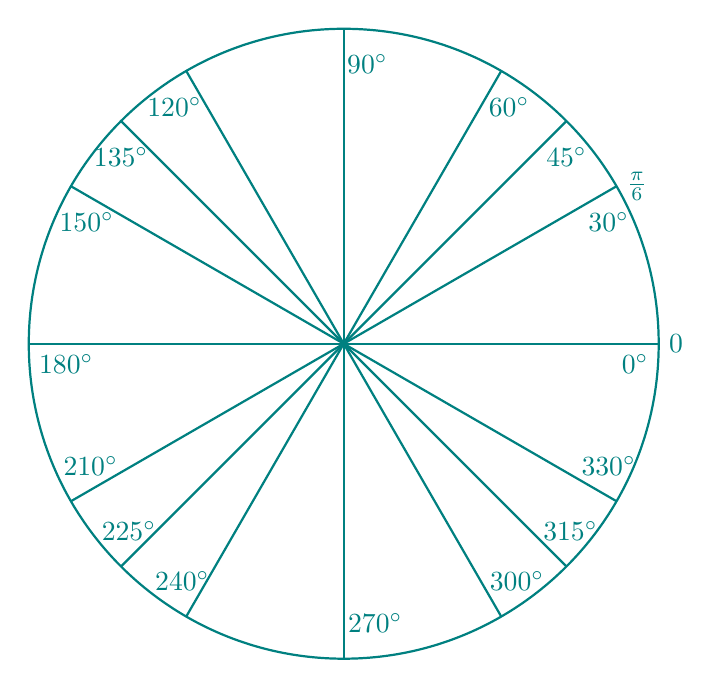
\begin{tikzpicture}
		\draw[thick, color = teal] (0,0) circle (4cm);
		\draw[thick, color = teal] (0,0) -- ({4*cos(0)},{4*sin(0)})
		node[pos = 1, anchor = north east] {$0^\circ$}
		node[pos = 1, anchor = west] {0};
		\draw[thick, color = teal] (0,0) -- ({4*cos(30)},{4*sin(30)})
		node[pos = 1, anchor = north, yshift = -0.2cm, xshift = -0.1cm] {$30^\circ$}
		node[pos = 1, anchor = west] {$\frac{\pi}{6}$};
		\draw[thick, color = teal] (0,0) -- ({4*cos(45)},{4*sin(45)})
		node[pos = 1, anchor = north, yshift = -0.2cm, xshift = -0cm] {$45^\circ$};
		\draw[thick, color = teal] (0,0) -- ({4*cos(60)},{4*sin(60)})
		node[pos = 1, anchor = north, yshift = -0.2cm, xshift = 0.1cm] {$60^\circ$};
		\draw[thick, color = teal] (0,0) -- ({4*cos(90)},{4*sin(90)})
		node[pos = 1, anchor = north, yshift = -0.2cm, xshift = 0.3cm] {$90^\circ$};
		\draw[thick, color = teal] (0,0) -- ({4*cos(120)},{4*sin(120)})
		node[pos = 1, anchor = north, yshift = -0.2cm, xshift = -0.15cm] {$120^\circ$};
		\draw[thick, color = teal] (0,0) -- ({4*cos(135)},{4*sin(135)})
		node[pos = 1, anchor = north, yshift = -0.2cm, xshift = -0cm] {$135^\circ$};
		\draw[thick, color = teal] (0,0) -- ({4*cos(150)},{4*sin(150)})
		node[pos = 1, anchor = north, yshift = -0.2cm, xshift = 0.2cm] {$150^\circ$};
		\draw[thick, color = teal] (0,0) -- ({4*cos(180)},{4*sin(180)})
		node[pos = 1, anchor = north west] {$180^\circ$};
		\draw[thick, color = teal] (0,0) -- ({4*cos(210)},{4*sin(210)})
		node[pos = 1, anchor = south, yshift = 0.2cm, xshift = 0.25cm] {$210^\circ$};
		\draw[thick, color = teal] (0,0) -- ({4*cos(225)},{4*sin(225)})
		node[pos = 1, anchor = south, yshift = 0.2cm, xshift = 0.1cm] {$225^\circ$};
		\draw[thick, color = teal] (0,0) -- ({4*cos(240)},{4*sin(240)})
		node[pos = 1, anchor = south, yshift = 0.2cm, xshift = -0.05cm] {$240^\circ$};
		\draw[thick, color = teal] (0,0) -- ({4*cos(270)},{4*sin(270)})
		node[pos = 1, anchor = south, yshift = 0.2cm, xshift = 0.4cm] {$270^\circ$};
		\draw[thick, color = teal] (0,0) -- ({4*cos(300)},{4*sin(300)})
		node[pos = 1, anchor = south, yshift = 0.2cm, xshift = 0.2cm] {$300^\circ$};
		\draw[thick, color = teal] (0,0) -- ({4*cos(315)},{4*sin(315)})
		node[pos = 1, anchor = south, yshift = 0.2cm, xshift = 0.05cm] {$315^\circ$};
		\draw[thick, color = teal] (0,0) -- ({4*cos(330)},{4*sin(330)})
		node[pos = 1, anchor = south, yshift = 0.2cm, xshift = -0.1cm] {$330^\circ$};
	\end{tikzpicture}
\end{center}

\subsection*{Opgave 5}
Brug enhedscirklen fra Opgave 4 samt Tabel \ref{tab:trig} til at udregne følgende værdier.
\begin{align*}
	&1) \ \sin\left(\frac{5\pi}{6}\right) &   &2) \  \tan\left(\frac{2\pi}{3}\right)   
	 &3) \ \cos\left(\frac{3\pi}{4}\right)   \\
	&4) \ \cos\left(-\frac{2\pi}{3}\right)  &   &5) \ \sin\left(\frac{11\pi}{6}\right) 
	   &6) \ \cos\left(-\frac{7\pi}{4}\right)   \\
	&7) \   \tan\left(-\frac{4\pi}{3}\right) &  &8) \  \sin\left(\frac{3\pi}{2}\right)  
	 &9) \ \cos\left(\frac{30\pi}{3}\right)   \\	
\end{align*}

\subsection*{Opgave 6}
Brug idiotformlen $\cos(x)^2 + \sin(x)^2 = 1$ til at bevise, at Tabel \ref{tab:trig} er sand. Du får brug for enhedscirklen for at indse, at $\cos\left(\frac{\pi}{3}\right) = 0.5$ samt $\sin\left(\frac{\pi}{6}\right) = 0.5$.

\subsection*{Opgave 7 (Med hjælpemidler)}
En cykel bevæger sig med en hastighed på 22m/s. Diameteren på cyklens hjul er 70cm. Bestem vinkelhastigheden for cyklens hjul i grader per sekund. 

\subsection*{Opgave 8 (Med hjælpemidler)} 
En katapult består af en 8 meter lang pind med et lod i den ene ende og et objekt, der skal kastes i den anden ende. Pinden står på en vippe, der er dobbelt så tæt på loddet, som den er på objektet, der skal kastes. Når objektet kastes, bevæger pinden sig med en vinkelhastighed omkring vippen på $802.5^\circ$ per sekund. Bestem objektets hastighed, når det kastes.
\subsection*{Opgave 9}
Vi skal bevise, at længden $k$ af en korde i en cirkel med radius $r$ henover en vinkel $\theta$ er givet ved
\begin{align*}
	k = 2r\sin\left(\frac{\theta}{2}\right).
\end{align*}
\begin{enumerate}[label=\roman*)]
	\item Brug Figur \ref{fig:kordebevis} til at bevise formlen for længden af en korde.
\end{enumerate}


\begin{figure}[H]
	\centering
	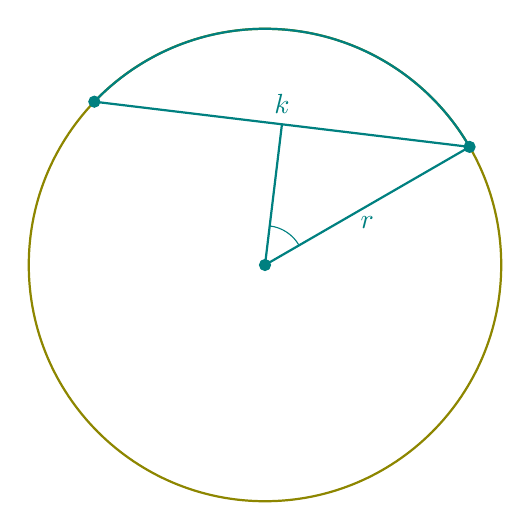
\begin{tikzpicture}
	\draw[color = olive, thick] (0,0) circle (3);
	\filldraw[color = teal] ({3*cos(30)}, {3*sin(30)} ) circle (2pt); 
	\filldraw[color = teal] ({3*cos(30+106.26)}, {3*sin(30+106.26)} ) circle (2pt); 
	\draw[color = teal, thick] ({3*cos(30)}, {3*sin(30)} ) -- ({3*cos(30+106.26)}, {3*sin(30+106.26)} )
	node[midway, anchor = south] {$k$};
	\draw[color = teal, thick] ({3*cos(30)}, {3*sin(30)} ) -- (0,0) node[midway, anchor = north] {$r$};
	\filldraw[color = teal] (0,0) circle (2pt);
	\draw[color = teal, thick] ({3*cos(30)}, {3*sin(30)} ) arc[start angle = 30, end angle = {30+106.26}, radius = 3];
	\draw[color = teal, thick] (0,0) -- ({1.8*cos(30+53.13)},{1.8*sin(30+53.13)});
	\draw[color = teal] ({0.5*cos(30)},{0.5*sin(30)}) arc[start angle = 30, end angle = {30+53.13}, radius = 0.5];
	\end{tikzpicture}
	\caption{Bevis for længde af korde}
	\label{fig:kordebevis}
\end{figure}